\documentclass[tikz,border=2pt]{standalone}
\usepackage{tikz}
\begin{document}
  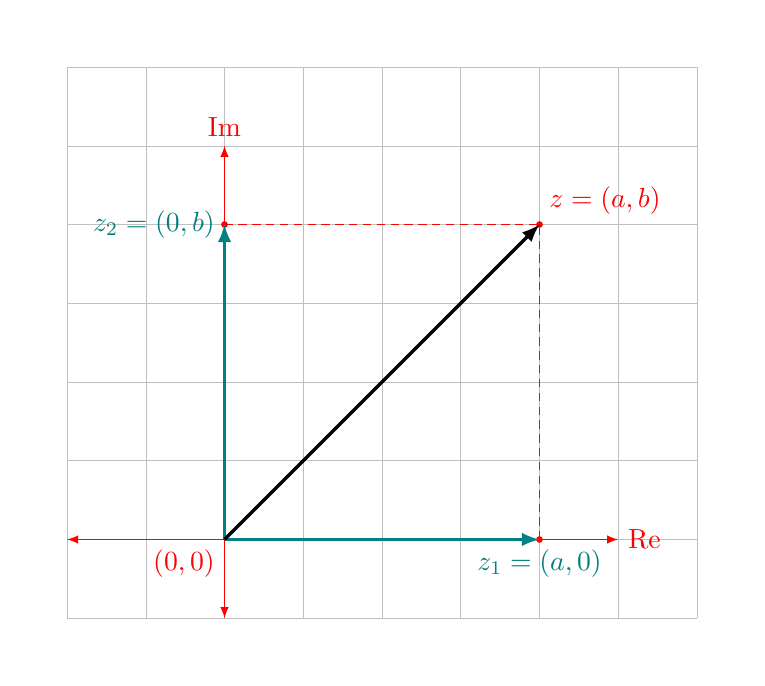
\begin{tikzpicture}
    \fill[white] (-2.5,-1.5) rectangle (6.5,6.5);
    \draw[lightgray,very thin] (-2,-1) grid (6,6);
    \draw (0,0) node[red,below left]{$(0,0)$};
    \draw[red,latex-latex] (-2,0) -- (5,0) node[right]{Re};
    \draw[red,latex-latex] (0,-1) -- (0,5) node[above]{Im};
    \draw[red,densely dashed] (4,0) -- (4,4);
    \draw[red,densely dashed] (0,4) -- (4,4);
    \filldraw[red] (4,4) circle(1pt) node[above right]{$z=(a,b)$};
    \draw (4,0) node[teal,below]{$z_1=(a,0)$};
    \filldraw[red] (4,0) circle(1pt);
    \draw[teal,very thick,-latex] (0,0) -- (4,0);
    \draw (0,4) node[teal,left]{$z_2=(0,b)$};
    \filldraw[red] (0,4) circle(1pt);
    \draw[teal,very thick, -latex] (0,0) -- (0,4);
    \draw[very thick,-latex] (0,0) -- (4,4);
  \end{tikzpicture}
\end{document}
